\section{The gem5 Simulator}

% Define "simulated perf" and simulator perf
% define guest, host, simulator, etc.

There is ``a new golden age for computer architecture''~\cite{HennessyPatterson-turingLect-isca18, HennessyPatterson-CACM19} driven by changes in technology (e.g., the slowdown of Moore's Law and Dennard Scaling) and ever increasing computational needs.
One of the first steps in research and development of new hardware architectures is software-based modeling and simulation.
The gem5 simulator~\cite{Binkert-gem5-2011} is currently one of the most popular academic-focused computer architecture simulation frameworks.
Since its publication in 2011, the gem5 paper has been cited over 3600 times\footnote{\url{https://scholar.google.com/scholar?q=gem5}}, and every year many papers published in the top computer architecture venues use gem5 as their main evaluation infrastructure.

The gem5 simulator~\cite{Binkert-gem5-2011} is an open source community-supported computer architecture simulator system.
It consists of a simulator core and models for a wide number of components from out-of-order processors, to DRAM, to network devices.
The gem5 project consists of the gem5 simulator\footnote{\url{https://gem5.googlesource.com/public/gem5}}, documentation\footnote{\url{https://www.gem5.org/}}, and common resources\footnote{\url{https://gem5.googlesource.com/public/gem5-resources}} that enable computer architecture research.

The gem5 project is governed by a meritocratic, consensus-based community governance document\footnote{\url{https://www.gem5.org/governance/}} with a goal to provide a tool to further the state of the art in computer architecture.
%The goal of gem5 is to provide a tool to further the state of the art in computer architecture.
The gem5 simulator can be used for (but is not limited to) computer-architecture research, advanced development, system-level performance analysis and design-space exploration, hardware-software co-design, and low-level software performance analysis.
Another goal of gem5 is to be a common framework for computer architecture research.
A common framework in the academic community makes it easier for other researchers to share workloads and models as well as compare and contrast their innovations with other architectural techniques.

The gem5 community strives to balance the needs of its three categories of users: academic researchers, industry researchers, and students learning computer architecture.
For instance, the gem5 community strives to balance adding new features (important to researchers) and a stable code base (important for students).
Specific user needs important to the community are enumerated below:
\begin{itemize}
    \item Effectively and efficiently emulate the behavior of modern processors in a way that balances simulation performance and accuracy
    \item Serve as a malleable baseline infrastructure that can easily be adapted to emulate the desired behaviors
    \item Provide a core set of APIs and features that remain relatively stable
    \item Incorporate features that make it easy for companies and research groups to stay up to date with new features and bug fixes as well as continue contributing to the project
    \item Additionally, the gem5 community is committed to openness, transparency, and inclusiveness.
\end{itemize}

In this paper, we discuss the current state of gem5.
We first discuss the past, present and future of the gem5 project and how to become a member of the gem5 community for researchers, students, and teachers in Section~\ref{sec:current-gem5}.
Then, we give an overview of gem5's main features available today describe and how to use gem5 for its main use case: computer architecture simulation~\ref{sec:main-features}.
Finally, Section~\ref{sec:changes} enumerates the major changes in gem5 in the past nine years since the initial release.

It has taken a huge number of people to make gem5 what it is today.
One of the goals of this paper is to recognize the hard work on this community infrastructure which is often overlooked.
To that end, we strive to include everyone who contributed to gem5 and document as many of the major changes as we can.
Section~\ref{sec:acks} acknowledges those contributors who are not authors of this paper and without whom gem5 would not be as successful.

\subsection{The past, present, and future of gem5}\label{sec:current-gem5}

The gem5 simulator was born when the m5 simulator~\cite{BinkertDHLSR06} created at University of Michigan merged with the GEMS simulator~\cite{MartinSBMXAMHW05} from University of Wisconsin.
These were two academic-oriented simulators, neither of which had an open development community (both simulators had their source available for free\footnote{\url{https://sourceforge.net/projects/m5sim/}}\footnote{\url{https://research.cs.wisc.edu/gems/home.html}}, but did not have a community-oriented development process).
Both of these simulators were quite popular on their own.
The GEMS paper has been cited over 1800 times and the m5 paper has been cited over 1000 times.

Since its initial release nine years ago the gem5 simulator has been wildly successful.
In this time, the use of gem5 has exploded.
Although not a perfect metric, as shown in Figure~\ref{fig:citations} the gem5 paper has received over 3600 citations according to Google Scholar.

\begin{figure}
    \centering
    \begin{subfigure}{0.28\linewidth}
      \centering
      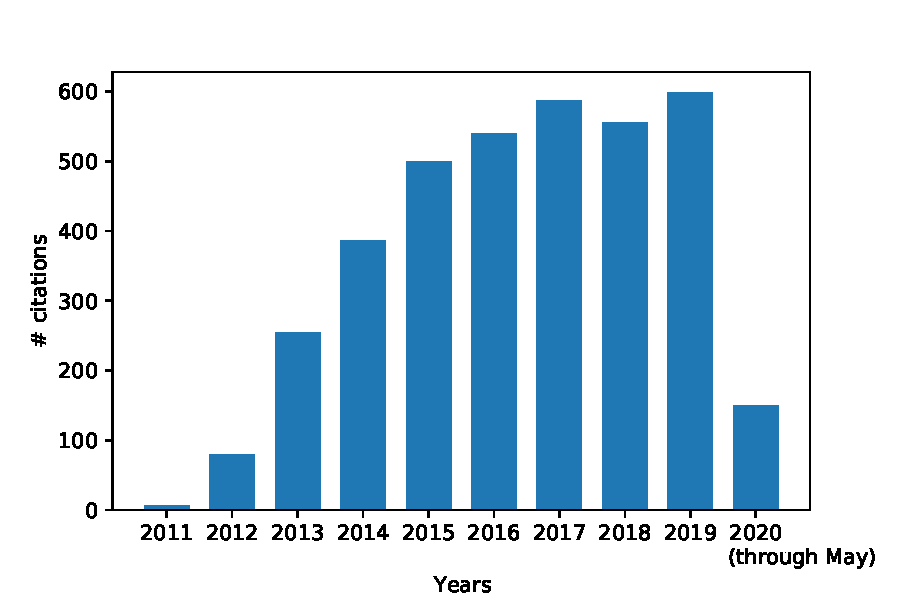
\includegraphics[width=\linewidth]{fig/gem5_citations}
      \caption{Number of citations}
      \label{fig:citations}
    \end{subfigure}
    \begin{subfigure}{0.28\linewidth}
      \centering
      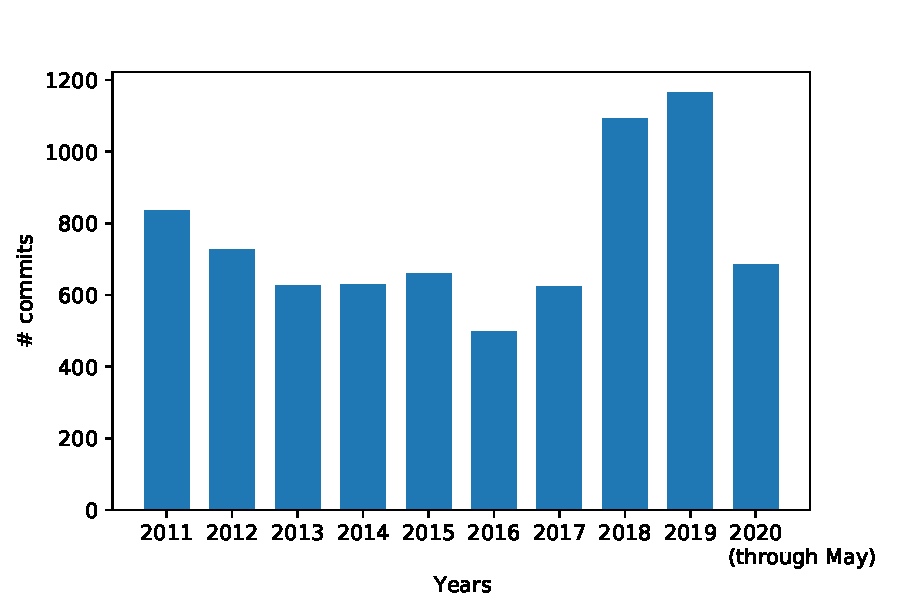
\includegraphics[width=\linewidth]{fig/gem5_commits}
      \caption{Number of commits}
      \label{fig:commits}
    \end{subfigure}
    \begin{subfigure}{0.28\linewidth}
      \centering
      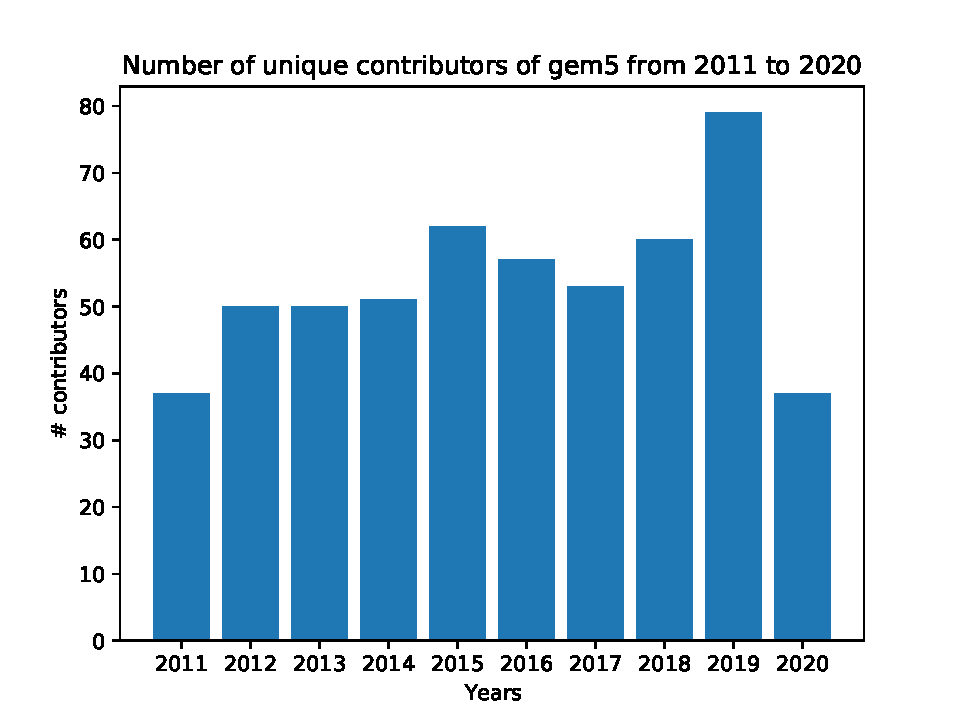
\includegraphics[width=\linewidth]{fig/gem5_contributors}
      \caption{Number of contributors}
      \label{fig:contributors}
    \end{subfigure}
    \caption{Number of gem5 citations, commits and contributors from 2011 to May 2020.}
    \label{fig:gem5_citations_commits_contributors}
\end{figure}

At the same time, the contributor community has also grown.
Figure~\ref{fig:commits} shows the number of commits per year and Figure~\ref{fig:contributors} shows the number of unique contributors per year.
These figures show that since the initial release of gem5 in 2011, development has been accelerating.

With this acceleration in use and development came growing pains~\cite{Power-gem5horrors-2015}.
The gem5 community was going through a shift, from a small project with most contributors from one or two academic labs, to a project with worldwide-distribution of contributors.
Additionally, given the growing user base, we could no longer assume that all gem5 users were also going to be main developers.

To solve the problems brought up by the expanding gem5 community, the gem5 project has made major changes in the past nine years.
We now have a formal governance structure, we have improved our documentation (see Section~\ref{sec:learning}), we have moved to a better distributed development platform, and we have improved our community outreach.

To institute a formal governance model, we followed the best practices from other successful open source projects.
We chose to institute a meritocratic governance model where anyone with an interest in the project can join the community, contribute to the project design and participate in the decision-making process.
The governance structure also defines the roles and responsibilities of members of the community including users, contributors, and maintainers.
We also formed a project management committee~(PMC) with a mix of industry and academic members to help ensure smooth running of the project.
%Importantly, members of the PMC do not have significant authority over other members of the community or of the direction of the project.

To simplify the contribution process, we have instituted many industry-standard development methodologies including providing a \verb|CONTRIBUTING| document in the gem5 source.
In the past, gem5 code contributions were managed with a number of esoteric software packages.
Now, all gem5 code is stored in a git repository\footnote{\url{https://gem5.googlesource.com/}}, code review is managed on gerrit\footnote{\url{https://gem5-review.googlesource.com/}}, we have continuous integration support (see Section~\ref{sec:testing}), our website is implemented with jekyll and markdown\footnote{\url{https://gem5.googlesource.com/public/gem5-website}}, and we have a Jira-based issue tracker\footnote{\url{https://gem5.atlassian.net/}}.

After transitioning to these more well known tools and improving our development practices, we have seen a further rise in the number of community contributors and using gem5 has become easier.
Continuous integration enables us to test every single changeset before it is committed.
This allows us to catch bugs \emph{before} they are committed into the mainline repository which makes gem5 more stable.
Similarly, by implementing a bug tracking system, we can track issues that affect gem5.
For example, in the first six months of using a bug tracker we have closed over 250 issues.

\subsubsection*{The future of gem5}
The future of gem5 is bright.
We are continuing to work with the community to define the roadmap for gem5 development for the next version of gem5, version 20.1, and beyond.
In the short term, we are excited about improvements to the underlying infrastructure of gem5 with better testing, refactoring of aging code (some of gem5's code is over 20 years old!), and adding well-defined stable APIs.
By defining stable APIs, we will make it easier for the community to build off of gem5.
For instance, the inter-simulator interface is currently being defined so that gem5 can be used in conjunction with other simulators (e.g., SST~\cite{RodriguesHemmert2011-sst, HsiehPedretti2012-sst-gem5}, SystemC (Section ~\ref{sec:systemc}), and many others).
We are also working on improving the interconnect model (Section~\ref{sec:garnet}), adding support for non-volatile memory controllers (Section~\ref{sec:nvm}), and a graphical user interface (GUI).

One of the most exciting features coming to gem5 is that we will provide the community with a set of \emph{publicly validated} models which will model current architectural system components including CPU cores, GPU compute units (CUs), caches, main memory systems, and devices.
Past research~\cite{butko2012accuracy, nowatzki2015architectural, endo2014micro, akram201686, asri2016simulator, akram2019validation, gutierrez2014sources, jo2018diagsim, tanimoto2017dependence, walker2018hardware} has shown that some gem5 models can be imprecise.
We strive for accuracy compared to real systems; however, since most systems are proprietary and complex, accuracy for all workloads will be difficult.
Thus, we will broadly advertise the relative performance, power, and other metrics when providing these models so users can make an informed decision when choosing their baseline configurations.
This will reduce the researcher's time spent on configuring baselines and allow them to concentrate more effort on analyzing and developing their novel research ideas.
The first step towards this goal of validated baselines is the gem5 resources repository described in Section~\ref{sec:resources}.

Finally, we are planning to publish an online \emph{Learning gem5} course based on an expanded version of the \emph{Learning gem5} material~\ref{sec:learning}\footnote{\url{http://www.gem5.org/documentation/learning_gem5/}}.
This course will cover how to get started using gem5, how to develop new models to be used in gem5, and the details of gem5's software architecture.
In addition to the online version of the course, we will continue to conduct tutorials and workshops at computer architecture and computer systems conferences.

However, the broader gem5 community is the most important part of gem5's future.
In the next section, we discuss how to become part of the gem5 community.

\subsection{Becoming part of the gem5 community}

As a reader of this paper, you are already becoming part of the gem5 community!
Anyone who uses gem5 or contributes in any way is part of the gem5 community.
Contributing can be as simple as sending a question on the gem5 mailing list\footnote{\url{http://www.gem5.org/mailing_lists/}} or as complex as adding a new model to the upstream codebase.
Below, we discuss some of the common ways to use gem5 and become part of the community.

\subsubsection{For researchers}

Currently, the most common gem5 use case is computer architecture research.
In this case, researchers download the gem5 sources, build the simulator, and then add their own device models on top of the models included in upstream gem5.
This use case requires deep knowledge of the core simulation frameworks of gem5.
However, we are working to make it easier to get started developing and researching with gem5 through efforts like the \emph{Learning gem5} materials and online course (Section~\ref{sec:learning}).

After using gem5 in their research, we encourage these users to contribute their improvements and fixes to gem5 back to the mainline codebase.
Not only does this improve gem5 for others, but it also makes reproducing research results easier.
Rather than managing many local changes and trying to keep up with new releases of gem5, when code is contributed upstream it is the responsibility of \emph{others in the community} to ensure that the code stays up to date.
Additionally the gem5 project employs a permissive BSD license to lower the barrier of contribution for both academic and industry researchers.

\subsubsection{For students and teachers}

The gem5 simulator can be used as a tool for teaching computer architecture as well.
Historically, there has been a very steep learning curve for using gem5 even for simple experiments.
However, we are improving the documentation for new users.

We will be continuing to improve gem5 with the goal of making it easier for both students and teachers to learn and teach computer architectures concepts.
For example, the new \emph{Learning gem5} material created for the online course will include a set of example exercises that we hope can be used in both undergraduate and graduate computer architecture courses.
Additionally, we are working to develop a new GUI-based front-end for gem5 and to develop known-good models that do not required deep knowledge of simulator internals to configure and use.

gem5 can be used in a computer architecture course by having the students download and build gem5 themselves or by providing them with a pre-built binary.
Then, the students can create different gem5 configurations which vary hardware parameters (e.g., issue width, cache associativity, etc.).
Finally, the students can explore the effects of these architectural changes on a wide array of common benchmarks and realistic applications from the gem5-resources repository (see Section~\ref{sec:resources}).

\subsection{gem5's main features}
\label{sec:main-features}

The gem5 simulator is mainly used to conduct computer architecture research.
In most cases, researchers have an application or benchmark for which they want to measure some \emph{statistics} under different hardware configurations.
For instance, they may be interested in the run time, the memory bandwidth, number of branch predictor mis-speculations, etc.
The gem5 simulator allows users to run applications and simulate the timing of hardware structures.
It contains models for the processor core (CPU), memory, and devices.

Although there are many computer architecture simulators, and many of these are open source with features that overlap with gem5, gem5 is a unique simulation infrastructure.
\begin{itemize}
    \item gem5 is \emph{dynamically configurable} through a robust Python-based scripting interface. Most other simulators are configured statically with flat text files (e.g., json) or at compilation time. On the other hand, gem5 allows users to simulate complex systems much more easily by using object-oriented Python scripts to compose simpler systems into more complex ones.
    \item gem5 is \emph{extensible} through a clean model API. The gem5 simulator has over 300 models and adding new models is straightforward and well documented.
    \item gem5 is a \emph{full system} simulator. Its high-fidelity models can support booting unmodified operating systems and running modified applications with cycle-level statistics.
    \item gem5 is a \emph{community-driven} and \emph{frequently updated} project. The gem5 community is thriving. Since its original release nine years ago, there have been over 250 unique contributors and over 7500 commits. Even in the last six months, gem5 has had over 850 commits and 50 unique contributors.
\end{itemize}

\begin{figure*}
  \centering
  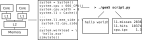
\includegraphics[width=0.7\linewidth]{fig/gem5-usage}
  \caption{How gem5 is used for computer architecture research. An example system is shown on the left, the sketch of a simulation script is shown in the middle, and the results of the gem5 simulation are shown on the right.}
  \label{fig:gem5-usage}
\end{figure*}

An overview of gem5's usage is shown in Figure~\ref{fig:gem5-usage}.
First, the user chooses a system to simulate (e.g., a two core system with two levels of cache shown on the left of Figure~\ref{fig:gem5-usage}).
Then, the user writes a Python script that describes the system under test by instantiating model objects (\verb|SimObjects| in gem5 terminology).
Each object has a number of parameters that the user can modify in their script by setting member variables of the Python objects.
This script is also used to control the simulator and can start the simulation, stop the simulation, save the simulation state, and complete other simulator interactions.
To execute the simulation, the user passes this Python script to the gem5 binary, which acts as a Python interpreter and executes the script.
This instantiates the system and runs the simulation as specified in the script.
The output of gem5 is the output of the application (e.g., standard output or the serial terminal in full system mode) and statistics for each of the simulated model objects.

Many of gem5's features are also useful for other computer systems and programming languages research (e.g., as a platform for developing JIT compilers~\cite{Shingarov2015-jit}).

The gem5 simulator is an ``execute-in-execute'' simulator.
Each operation (e.g., instruction, memory request, I/O operation) is functionally completed at the point that the timing simulation specifies.
For instance, each instruction is executed when it is in the execute stage of the pipeline.
This is in contrast to trace-based and execute-ahead simulators.
The main benefit of execute-in-execute is when running applications whose code path depends on the timing of multiple threads or I/O.
Trace-based or execute-ahead simulation may hide potential behaviors and produce different timing results than real hardware.

To enable modularity, gem5 separates the \emph{functional} execution from the \emph{timing} in most of its models.
For instance, each of gem5's CPU models can be used with any ISA as the ISA's functional implementation is separate from the CPU timing model.
This separation allows gem5 to create checkpoints during execution, fast-forward to the region of interest using low fidelity models, and introspection from the simulator into the simulated system at runtime.

\begin{figure*}
  \begin{subfigure}{0.28\linewidth}
    \centering
    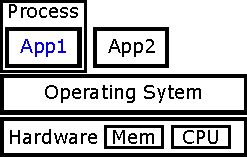
\includegraphics[width=\linewidth]{fig/gem5-fs-normal}
    \caption{The common hardware/software abstraction layers.}
    \label{fig:gem5-fs-normal}
  \end{subfigure}
  \hfill
  \begin{subfigure}{0.28\linewidth}
    \centering
    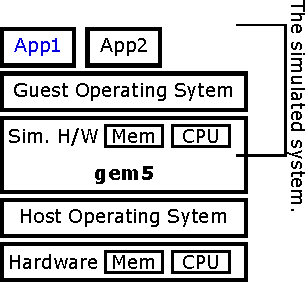
\includegraphics[width=\linewidth]{fig/gem5-fs-fs}
    \caption{The hardware/software abstraction layers when using gem5 in full system simulation mode.}
    \label{fig:gem5-fs-fs}
  \end{subfigure}
  \hfill
  \begin{subfigure}{0.28\linewidth}
    \centering
    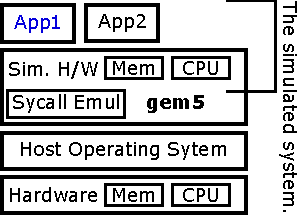
\includegraphics[width=\linewidth]{fig/gem5-fs-se}
    \caption{The hardware/software abstraction layers when using gem5 in system call emulation mode.}
    \label{fig:gem5-fs-se}
  \end{subfigure}
  \caption{A comparison of gem5's different modes of operation.}
  \label{fig:gem5-fs}
\end{figure*}

The gem5 simulator can be used in two different modes: full system simulation or system call emulation (syscall emul or SE-mode).
Figure~\ref{fig:gem5-fs} shows the hardware/software abstraction layers in each of these cases.
In \emph{full system} mode, gem5 can boot a full Linux-based operating system (e.g., Ubuntu 20.04).
After booting the guest OS, the researcher can run the application of interest to generate statistics.
In system call emulation mode, the gem5 simulator itself emulates the operating system.
The support for Linux system calls has been greatly improved recently (see Section~\ref{sec:se-mode}).
SE-mode ignores the timing of many system-level effects including system calls, TLB misses, and device accesses.
Thus, researchers should use caution when running experiments in SE-mode and ensure that ignoring system-level effects will not change the results of the experiments.

% Could define benchmark, system under test, guest, host, etc. here.

\subsubsection{gem5 design}

The gem5 simulator is a cycle-level computer system simulation environment.
At its core, gem5 contains an event-driven simulation engine.
On top of this simulation engine, gem5 implements a large number of models for system components from CPUs (out-of-order designs, in-order designs, and others), memories (such as DDR3/4, GDDR5, HBM, and HMC), on-chip interconnects, coherent caches, I/O devices, and many others.
Many of these different models are shown in Figure~\ref{fig:gem5-big-picture}.
The gem5 project also contains tests to help find bugs, a complex and feature-rich statistics database, and a Python scripting interface to describe systems under test and run simulations.

\begin{figure*}
  \centering
  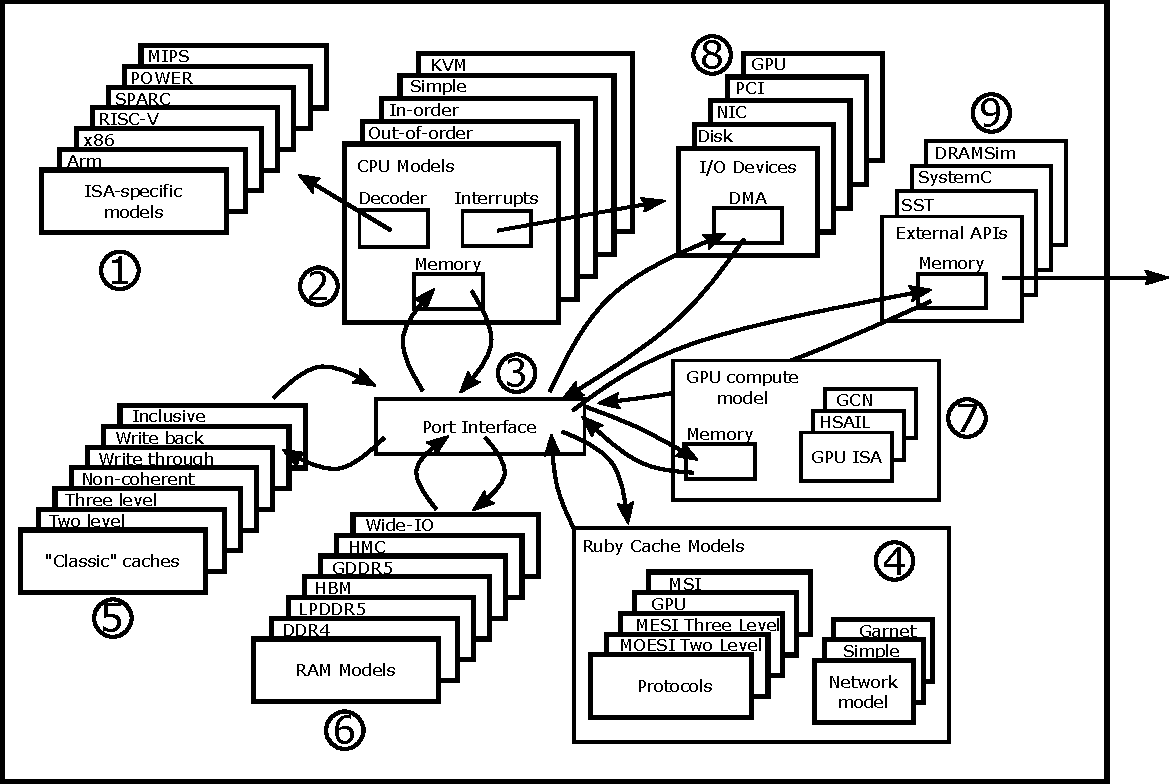
\includegraphics[width=\textwidth]{fig/gem5-big-picture}
  \caption{An overview of gem5's architecture. Its modular components allow any of each model type to be used in system configuration via Python scripts. Users can choose the fidelity of the memory system, CPU model, etc. while being able to select any ISA, devices, etc. The port interface allows any memory component to be connected to any other memory component as specified by the Python script. Details of each of these simulator components are discussed in Section~\ref{sec:main-features}}
  \label{fig:gem5-big-picture}
\end{figure*}

The gem5 simulator has modular support for multiple ISAs (see Figure~\ref{fig:gem5-big-picture}~\textcircled{1}).
The gem5 simulator currently supports Arm, GPU ISAs, MIPS, Power, RISC-V, SPARC, and x86.
These ISAs not only include the details to execute each instruction, but also the system-specific devices necessary for full system simulation.
There is robust full system support for Linux on Arm and x86.
Additionally, many other ISAs have some level of full system support.

All of these ISAs can be used with any of gem5's CPU models as the CPU models are designed to be ISA-agnostic (Figure~\ref{fig:gem5-big-picture}~\textcircled{2}).
Four different CPU models are included which span the fidelity-performance spectrum.
The gem5 simulator contains ``simple'' CPU models that can be used for memory system studies or other studies that do not require high-fidelity execution models.
Additionally, gem5 contains a detailed in-order CPU model (the ``minor'' CPU) and an out-of-order CPU model (the ``O3'' CPU).
Finally, gem5 includes a CPU model that is based on the kernel virtual machine (KVM) that leverages hardware virtualization to execute \emph{at native speeds}~\cite{full-speed-ahead} resulting in minimal simulator overhead compared to native execution.
Although the KVM CPU model can execute at native speed, it does not model the timing of execution or memory requests.
The KVM-based CPU model can be used for fast-forwarding to the region of interest, sampled simulation, and fast-forwarding to checkpoint locations.

To connect the different compute, memory, and I/O device models gem5 provides a modular port interface which allows any component that implements the port API to be connected to any other component implementing the same API (Figure~\ref{fig:gem5-big-picture}~\textcircled{3}).
This allows models designed for one system to be easily used in other system designs.

There are two different cache systems in gem5: Ruby (Figure~\ref{fig:gem5-big-picture} \textcircled{4}), which models cache coherence protocols with high fidelity; and the ``classic'' caches (Figure~\ref{fig:gem5-big-picture}~\textcircled{5}), which lack cache coherence fidelity and flexibility.
Ruby enables user-defined cache coherence protocols and gem5 includes many different protocols out of the box.
%There are now 12 unique protocols including GPU-specific protocols~\cite{viper}, research protocols like token coherence~\cite{token-coherence} and region-coherence protocols~\cite{PowerBasu2013-hsc}, and teaching protocols~\cite{coherence-primer}.
Users can also choose to use a simple network model or the detailed Garnet model~\cite{garnet-2} when using Ruby caches which offers cycle-level detail for the on-chip network.

The classic caches have a single hard-coded hierarchical MOESI coherence protocol.
However, this cache model is easily composable allowing users to construct hierarchical cache topologies without worrying about the details of the coherence protocol.
Both Ruby and the classic caches can be used with any CPU model, any ISA, and any memory controller model.

The gem5 simulator also includes an event-driven DRAM model (Figure~\ref{fig:gem5-big-picture}~\textcircled{6}).
This DRAM model is easily configurable with the timing parameters for a variety of different DRAM controllers including DDR3, DDR4, GDDR, HBM, HMC, LPDDR4, LPDDR5, and others.
Although this is not a cycle-accurate DRAM model like DRAMSim~\cite{wang_05, dramsim2, dramsim3} or Ramulator~\cite{yoongy_16}, it is nearly as accurate while providing more flexibility and higher performance~\cite{HanssonAgarwal2014-gem5DRAM}.

In addition to CPU models, gem5 also includes a cycle-level compute-based GPU~\cite{GutierrezBeckmann2018-amdAPU, Ta2019gputesting} (Figure~\ref{fig:gem5-big-picture}~\textcircled{7}).
This GPU model does not support graphics applications, but supports many compute applications based on the heterogeneous system architecture (HSA) and ROCm runtime.
The GPU model is based on AMD's Graphics Core Next (GCN) architecture~\cite{gcnWhitepaper, gcn3Manual}.
The GPU model has a modular ISA similar to the CPU model in gem5, and can be extended to support other GPU ISAs in the future. Additionally, gem5 contains support for a functional-only GPU model to enable simulating applications that depend on graphics APIs but do not depend on graphics performance~\cite{nomali}.

An important component to full system simulation is supporting I/O and other devices (Figure~\ref{fig:gem5-big-picture}~\textcircled{8}).
Thus, gem5 supports many system-agnostic devices such as disk controllers, PCI components, Ethernet controllers, and many more.
There are also many system-specific device models such as the Arm GIC and SMMU, and x86 PC devices.

Finally, gem5 has been integrated with other computer architecture simulator systems to enable users with models in other simulator systems to use gem5's features (Figure~\ref{fig:gem5-big-picture}~\textcircled{9}).
For instance, gem5 has been integrated with the Structural Simulation Toolkit (SST)~\cite{RodriguesHemmert2011-sst, HsiehPedretti2012-sst-gem5}, which uses gem5's detailed CPU models in conjunction with SST's multi-node modeling capabilities.
DRAMSim~\cite{wang_05, dramsim2, dramsim3} which provides a cycle-accurate DRAM models has also been integrated with gem5.
Additionally, the IEEE standard SystemC API~\cite{menard2017-system-systemc} has been integrated to enable users with SystemC models to use them as gem5 components (see Section~\ref{sec:systemc} for more details).
